\chapter{Social Engineering}
First of all, we should dead with what sociology really is, then we
will master the vocabulary to be able to put a name on phenomenons,
and then we will deal with social engineering. We will apply some
sociological theories to think of a new way to perceive and represent
the complex relationships among machines and human beings.
\section{Sociology}
Let's kick off with a definition of sociology.

\begin{boxH}
  Sociology is the \textbf{science of social phenomena} subject to
  natural and invariable laws, with the goal of discovering these
  laws.

  - Auguste Comte, 1839
\end{boxH}
The important point is not the definition, but the fact the definition
contains many information about the cultural environment from which it
comes. If you think about it, the definition focuses on the scientific
method, which tries to quantify something in a deterministic fashion,
becase one believe that all the necessary informations are already
there. But natural laws are more complicated than these and human laws
are even more complicated. 

To sum this up, first, one can quantify social interactions, today we
do apply maths and statistics to social facts. Second there's a sort
of cause and effect relationship between social phenomena: just as at
that time they believed that nature was describable in this way, they
came up with the idea that society could be as well.

Another definition of sociology is the following:
\begin{boxH}
  Sociology is the study of human social life, groups, and societies.
  - Antony Giddens
\end{boxH}
As you can see, the scope of the definition was quite reduced.

There are also other figures that are important to keep in mind. The
first one is German sociologist and economist Max Weber, because he
guides us in understanding two key aspects of sociological inquiry.
First, it is \textbf{evolutive}: We live in a context of digital and
analogical interactions in which, if you don't take a stand for
something or for somebody, it means you're out of the debate. If you
think about it, social media algorithms have been coded in order to
emphasise this sort of polarisation effect, because the more polarised
the debate, the more engaged the debate becomes, which makes sense for
an economical standpoint, and this kind of interaction is becoming the
natural of the way we interact. The second lesson is that the
\textbf{uncertainty of data} is the only certainty we have. There
might be systemic errors in your data sets, accidental errors, and
they are due to the sometimes the impossibility to have direct access
to some sort of phenomenon (think for instance about criminality). The
fact that they are somehow at least partly accessible limits the scope
of the conclusions you are reaching. Even biases and subjectivity are
a problem, for instance, one reinvents the past when one tries to 
recall it, which is just the way our brain works.

The second relevant figure is Charles Wright Mills, a sociologist from
the US, the 50s and the 60s, the one who studied the white collars.
The key concept is the \textbf{sociological imagination}, which is the
ability to see when you want to social phenomena through the eyes of
scientific inquiry, not through common sense and stereotypes.



\subsection{Basic Sociological Vocabulary}

Sociology uses specific terms to describe the elements of society and
social behavior. Below are key concepts:

\textbf{Norms} are the rules and expectations by which a society
guides the behavior of its members. With members we refer to social
actors, which can be individuals, groups, or institutions. After all,
sociology uses theatrical metaphors to describe the interactions
within a society. So, norms are sets of rules that you are given
because you are recognised as a member, as an actor within a context,
a society. There are mainly two types of rules. Explicit norms and
implicit, or tacit, norms. Cyber criminals rely mostly on the latter 
ones, because they can be broken more easily. After all, they are
invisible to newcomers, and they are not written down, and they have
to be learned by experience.

\textbf{Values} refer to collective ideas about what is good,
desirable, and proper. Those are tricky elements, because the more
social they are, the less they seem to be, because, if a set of values
is very well spread within a group, each member of the group feels
like the values are obvious.

\textbf{Role} encompasses the set of norms, behaviors, and
expectations associated with a particular social status or position
within society. Roles guide how individuals are supposed to act and
interact with others in specific contexts. As described before, they
are strictly connected with the idea of playing the game or acting
society. We are usually more than a role, but we decide to show only 
a part of ourselves according to the context we are in. Roles are not
self-assigned, they are recognised by the others, and indeed,
sometimes when you feel you are not recognized in one role, you feel
uncomfortable.

\textbf{Social Structure} is the organized pattern of social
relationships and social institutions that together constitute
society.

\textbf{Culture} consists of shared beliefs, values, and practices. In
the end, humankind was able to organize social interactions against
chaos. That's why we can speak of societies, no matter how simple,
small or very complex and big they are. But they are very well
structured.

\subsection{The social iceberg}
To conclude this sociological journey, consider the image of an
iceberg—a fitting metaphor for social relations. Above the surface, we
find two dimensions. The first relates to corporality: our body,
nervous system, and senses help us perceive and interact with the
world. However, our senses are not foolproof; they can mislead us.
Hallucinations and memory distortions, for instance, demonstrate the
limits of our perception. Witness accounts of even simple events, like
a car accident, often differ significantly from each other and from
camera footage. This highlights how imperfect and subjective our
senses are—they are both gateways to the environment and sources of
error.

The second dimension involves processing sensory input through our
mental filters: past experiences, memories, learning, and
adaptability. These filters shape how we interpret the world and
decide how to act—or not to act. Sociologically, both action and
inaction are forms of behavior, influenced by this interplay of
perception and processing.

Below the surface of the iceberg lies a deeper realm of human
experience. This includes the mental "autopilot" we rely on to
navigate most of our daily activities. We don't constantly
"meta-think" or reflect on every action, like sitting in a chair or
walking. These routines are built on assumptions that rarely fail
us—until they do. When something disrupts our expectations, it forces
us to pause, question, and adjust. This reflects the philosopher
Hume's insight: we assume the sun will rise tomorrow because it always
has, but that certainty is not guaranteed.

Additionally, from birth, we begin absorbing knowledge through a
process sociologists call primary socialization. Caregivers teach
us how to express needs, interact with others, and adapt to our
environment. Early lessons—both instinctive and taught—form the
foundation of our behavior.

As we grow, secondary socialization takes over, enriching our
"autopilot" with experiences from school, friendships, work, and
culture. These interactions shape our social network, values, and
identity. From the music we enjoy to the relationships we build, this
ongoing process continually informs how we navigate and understand the
world.

\begin{figure}[H]
  \centering
  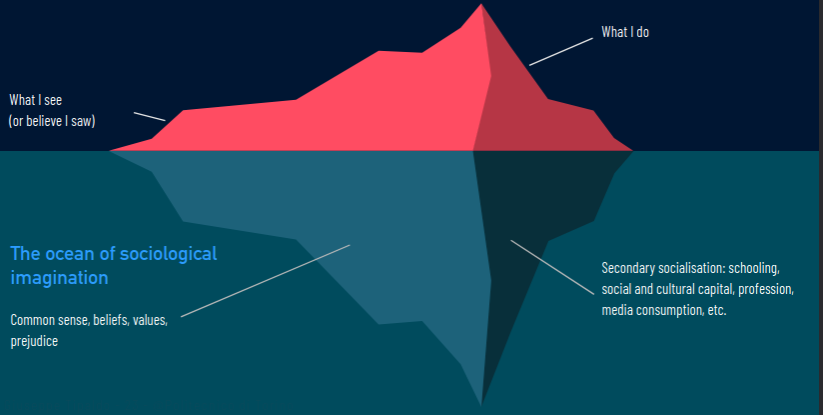
\includegraphics[width=0.5\textwidth]{img/sociology iceberg.png}
\end{figure}

\section{Vocabulary}
In general it is important to provide a clear definition of complex
phenomena to be able to apply more then a label to them. As such, we
will try to analyze different attempts to give a name to cyber
criminal activities. During the years, many definitions have been
provided, meaning that we need a way to classify them too.

\begin{boxH}
  One of the leading factors leading to difficulties in estimating
  cybercrime is exactly the fact that we don't have very well formed
  definitions nor a rigorous classification method.
\end{boxH}

The wider and richer the vocabulary, the more complex the thoughts you
can make, you can formulate.

We begin with the period from 1995 to 2000, during which the term
"cybercrime" was not even the dominant word used in discussions
related to the field. This stands in stark contrast to the following
window, 2001 to 2018, when "cybercrime" emerged as the most frequently
used term in scientific literature. It’s worth noting that 30 years
ago, there wasn’t even a widely agreed-upon term to describe
cybercrime in a scientific context. 

While 30 years might seem like a long time, it’s relatively brief in
the grand scheme of scientific progress. At the same time, it
represents a significant period during which research and terminology
have evolved. For instance, efforts to classify the various forms of
cybercrime often result in taxonomies that, no matter how
comprehensive, fall short of fully bridging the gap between
theoretical frameworks and real-world occurrences.

From such classifications, it becomes evident that creating broader
categories or groups can be helpful. These allow for more efficient
communication and problem-solving without the need to enumerate every
specific instance when referring to a broader class or subclass of
cybercrime.

\begin{figure}[H]
  \centering
  \includegraphics[width=0.7\textwidth]{img/cybercrime
  definitions.png}
  \caption{Organizational definitions of cybercrime.}
\end{figure}

As you can see, the definitions are quite different from each other,
some are broader, some are more specific.

There are several attempts to try and make it more clear and try to
classify those definitions in order to make it simpler to understand
for those maybe who lack some tech knowledge about cybersecurity. For
example, one proposal is to adopt a sort of categorical approach to
the systematization of definitions. A categorical approach is a 
systematic way to classify things, and with this approach we can
discern between cyber-enabled crimes and cyber-dependent crimes. 
\textbf{Cyber-enabled} crimes are traditional crimes that predate the
advent of the technology, and are now facilitated or have been made
easier (i.e., enabled) by cyber technology. Crimes range from
white-collar crime to drug trafficking, to online harassment,
terrorism and beyond.

\textbf{Cyber-dependent crimes} are crimes that arose with the advent
of technology and cannot exist (i.e., dependent) outside of the
digital world, e.g., hacking, such as ransomware attacks or
hacktivism.
